\documentclass{article}
\usepackage[utf8]{inputenc}
\usepackage{amsmath}
\usepackage{graphicx}
\usepackage{geometry}
\usepackage[colorlinks=true]{hyperref}
\usepackage{cleveref}
\usepackage{algorithm}
\usepackage{algpseudocode}
\graphicspath{ {./images/} }
\setlength{\parindent}{0pt}

\title{Dynamics of ``problem-place'' disease spread}
\author{}
\date{}

\begin{document}

\maketitle

\begin{abstract}
Disease transmission is often not homogeneous: a small
number of infected individuals are responsible for a disproportionately
large number of subsequent infections. 

This is certainly the case in COVID-19, in which 20\% of infections may cause
as many as 80\% of secondary infections[citation?].
However, our mechanistic understanding of this phenomenon – "super-spreading" –
is limited[citations?].

Here we introduce and analyze
a model of an outbreak with super-spreading via "problem-place" locations:
disease spreads homogeneously throughout the population at a low rate, but
spreads rampantly at certain locations (bars, restaurants, churches, etc.)
that individuals visit daily with their own fixed probabilities.

Compared to homogeneous dynamics, outbreaks are less
likely to happen but are accelerated when they do occur; causing larger
outbreaks in some cases, but paradoxically smaller and less severe outbreaks 
in moderately to highly infectious diseases.
\end{abstract}


After the SARS pandemic in 2005, researchers noted that disease transmission
was not homogeneous: some small number of infected individuals – coined
"super spreaders" – were responsible
for a disproportionately large number of subsequent infections.[2005 nature citation]
Subsequent research noted a similar pattern in other diseases: between
15\% to 20\% of infected individuals were led to 75\% to 85\% of later infections
in diseases as diverse as (examples). [2006 super spreading]. 
The COVID-19 pandemic follows a similar pattern: 15\% of super-spreading-
infected individuals cause 80\% of later infections.

Research into the dynamics of disease outbreaks with superspreading has
been mostly limited to models in which some "super spreading" individuals
are simply more infectious – either because of greater biological infectiousness
(higher viral load, larger lung capacity, etc.) or greater network connectivity.
But this doesn't match what we understand about the COVID-19 pandemic: 
individual infectiousness doesn't seem to vary all that much [citation of this].
And while certainly individuals'
connectivity varies, we know that transmission of COVID is centered around
certain "problem places": bars, restaurants, churches, etc. [problem place paper].

At the same time, recent work has developed a description of human movement
that quantifies a distribution of the frequency with which
people visit different places in urban settings. Specifically; 

Here we introduce the risk-structured "problem-place" SIR model in which
each individual has a fixed "risk" probability of visiting the problem-place
per unit time where disease spreads with very high transmission rate, while
simultaneously disease spreads with low transmission rate through
homogeneous community spread. We use three versions of this model – one agent-based
computational model, a differential equation model and a difference equation model –
to investigate how the theoretical dynamics of such disease spread differ from
the unstructured homogeneous SIR model, in particular:
- the likelihood of an epidemic outbreak upon introduction to a subpopulation
- the peak (largest number of simultaneously infected inviduals), and
- the total number of infected individuals across the outbreak

We find that problem-place dynamics make an outbreak less likely in
nearly all cases. When there is an outbreak, we see an acceleration in
both the early growth of the disease and its later decay. When
average infectiousness is low ($\mathcal{R}_0 < 1.2$) this causes a higher peak and
larger final size, when average infectiousness is moderate ($\mathcal{R}_0 1.2 - 2.0 $), it causes
a higher peak but smaller final size of outbreaks, and when infectiousness is
high ($\mathcal{R}_0 > 2$) it causes a lower peak and final size.



\section{Methods}

We use three versions of the same model to investigate problem-place risk
structure.

\subsection{Agent Based Model}

N individuals (typically set to 1,000) are initialized with risk values
$\rho_i$, $i \in [0, N]$ drawn independently from a fixed risk distribution.
These values never change for an individual.

One individual is chosen at random and set to infected.

Then we run the following loop:
\begin{verbatim}
until no individuals are infected:
	for i in [1, N]:
		roll a random number r in [0, 1]
		if r < rho_i:
			individual[i].takes_risk = True

	# problem place spread
	for i in [1, N]:
		if individual[i].status == INFECTED && individual[i].takes_risk:
			for j in [1, N]:
				if individual[j].status == SUSCEPTIBLE && individual[j].takes_risk:
					roll random number r in [0, 1]
					if r < beta_p:
						individual[j].status == INFECTED_NEXT

	# community spread
	for i in [1, N]:
		if individual[i].status == INFECTED:
			for j in [1, N]:
				if individual[j].status == SUSCEPTIBLE:
					roll random number r in [0, 1]
					if r < beta_c:
						individual[j].status == INFECTED_NEXT

	# recovery and new infections
	for i in [1, N]:
		if individual[i].status == INFECTED:
			individual[i].status = RECOVERED

	for i in [1, N]:
		if individual[i].status == INFECTED_NEXT:
			individual[i].status = INFECTED
\end{verbatim}

\subsection{Integrodifferential Model}




\subsection{Models}

\begin{itemize}
\item SIR is used throughout
\item ABM pseudocode
\item differential equation system
\item difference equation system
\end{itemize}

\subsection{Riskiness Distributions}

See \Cref{fig:risk_distributions}.


\begin{figure}
\centering
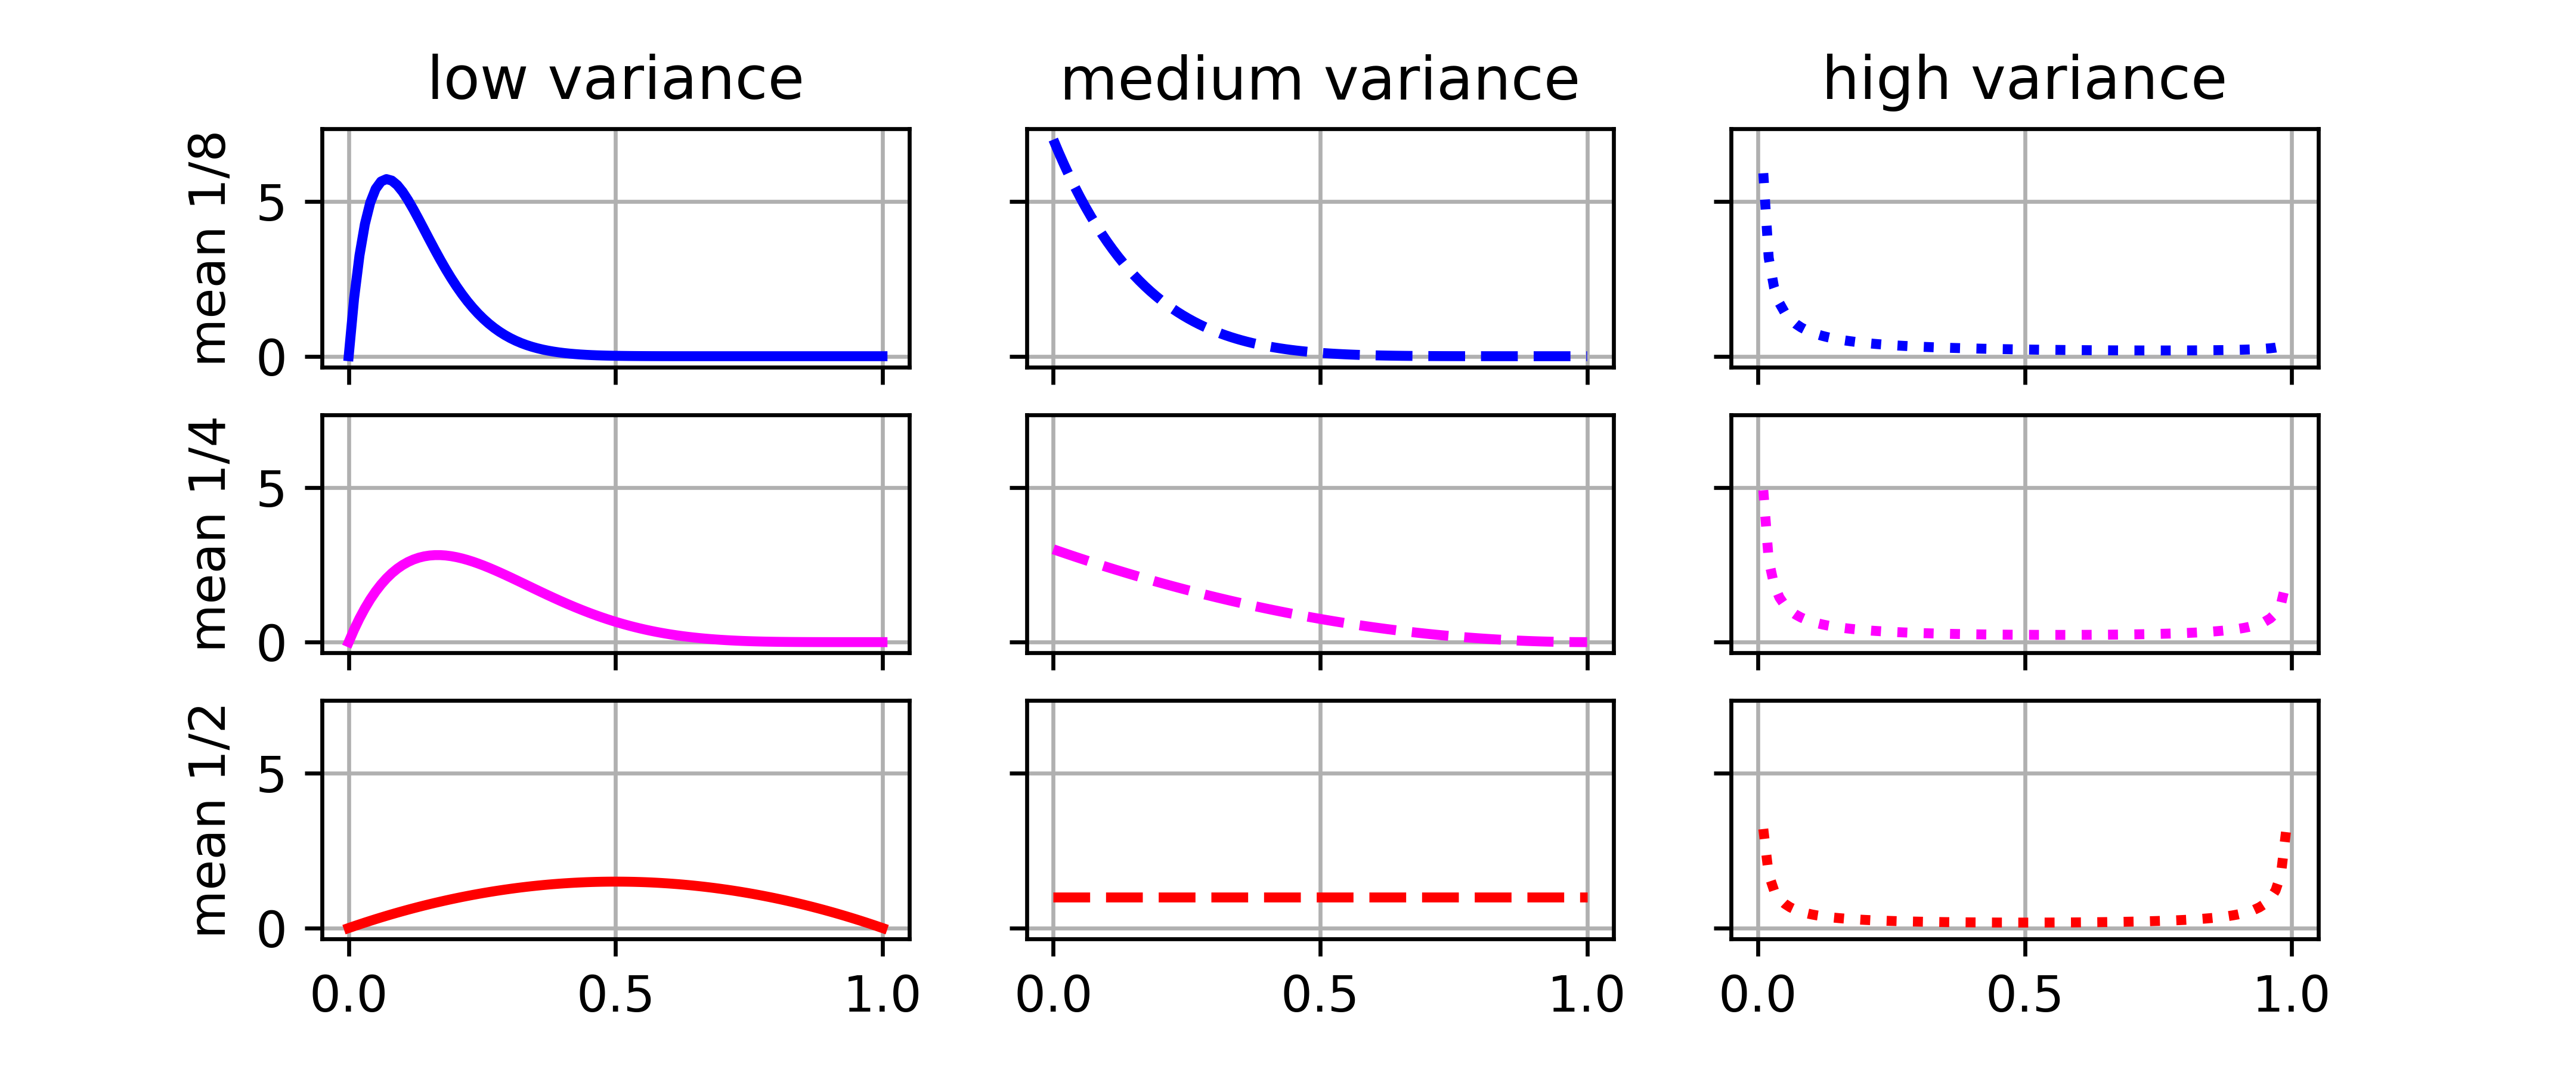
\includegraphics[width=\textwidth]{risk_distributions}
\caption{\textbf{Risk distributions of the initial population:} the top row
shows distributions in which \textit{on average} 1/8th of the population
goes to the problem-place per week which increase in variance from left to
right. The second row shows the same with mean 1/4, and the last row mean 
1/2. We don't consider higher means – if more than half of the population
spends time in the problem place per week, we start to approach the homogeneous
case. }
\label{fig:risk_distributions}
\end{figure}

\subsection{Basic Reproduction Number}

$$\mathcal{R}_0 = \mathcal{C}_0 + \mathcal{P}_0$$


\section{Results}
\subsection{Extinction Probability}


% Define: What is disease extinction?
How does extinction probability change in the problem place model?\\

We consider three scenarios: problem place spread is responsible (initally)
for 25\%, 50\% or 75\% of total disease spread. For each, we vary $\mathcal{R}_0$
from 0 to 8, and run a simulation 1000 times. One individual chosen
at random becomes infected and we run the simulation until all infeceted
individuals have recovered and record this total number of infected individuals.\\

These numbers are genarally bimodal – with simulations
ending at either 20 or fewer total recovered, or greater than 500 total
recovered – so we can categorize each simulation as containing an extinction
or an outbreak (using a threshold of 50 total recovered).\\

These results are all shown in \Cref{fig:extinction_results} for each of the riskiness
distributions discussed in the introduction.\\


\begin{figure}
\centering
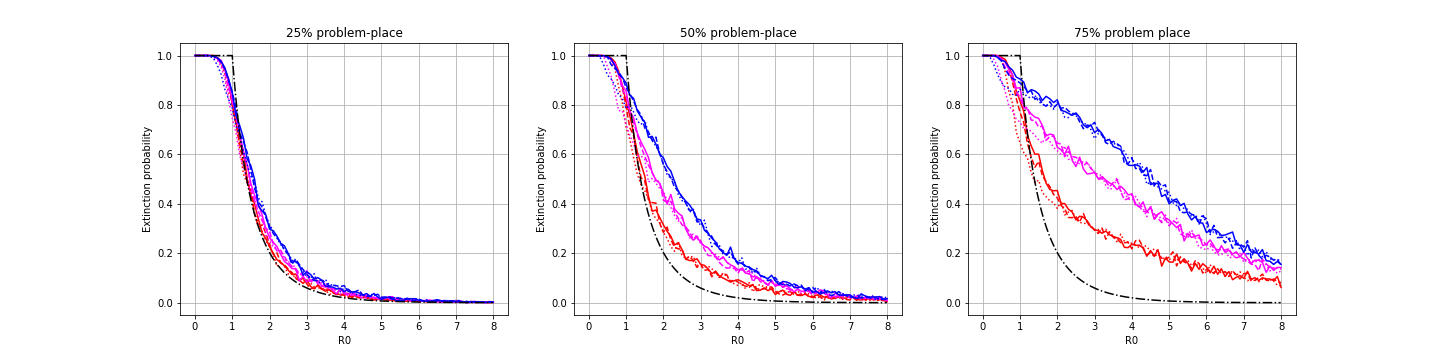
\includegraphics[width=\textwidth]{extinction_results}
\caption{\textbf{Simulated extinction probabilities:} we start with a population
of N=1000 susceptible agents and choose one at random to become infected. We
run the simulation until no agents are actively infected and then
decide based on a threshold (N=50 recovered agents) whether there
was an outbreak or disease extinction. We repeat 1000 times to determine
"extinction probability." We do this for each of the nine risk distributions
in \Cref{fig:risk_distributions} and the homogeneous case and for
$\mathcal{R}_0$ varying from 0 to 8; using 25\% (left), 50\% (middle) and 
75\% (right) problem-place spread.}
\label{fig:extinction_results}
\end{figure}



We find that higher problem place spread means an outbreak is overall less
likely (extinction probability is greater). We find that this effect is
more pronounced the lower the mean risk taking in the population. And we see,
surprisingly, that the effect is exactly the same \textit{between} scenarios
with the same mean riskiness even if their distributions otherwise vary
significantly (lines of the same color overlap).


To explain these results, we approximate the simulation with a branching process
(derivation is shown in the appendix)
and find that we can compute the "extinction" probability of a given simulation
$\tau$ as:

\begin{equation}
\tau = ... \tau
\label{eqn:extinction}
\end{equation}


\begin{figure}
\centering
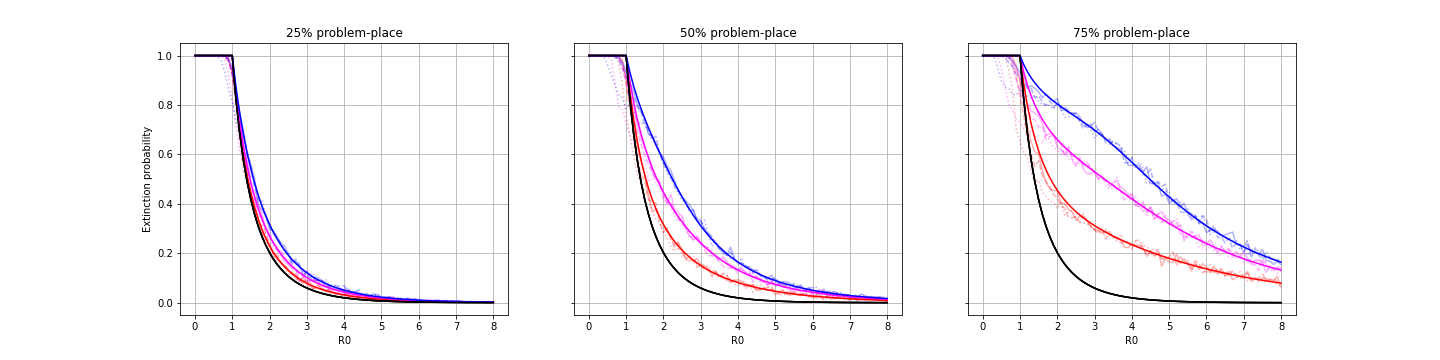
\includegraphics[width=\textwidth]{extinction_explained}
\caption{\textbf{Predicted extinction probabilities:} we show predictions
according to \Cref{eqn:extinction} (solid) over simulation
results from \Cref{fig:extinction_results} (faint).}
\label{fig:extinction_explained}
\end{figure}




These predictions are shown in \Cref{fig:extinction_explained} compared
to the simulated results from \Cref{fig:extinction_results}, showing
great agreement. So what does this tell us?\\


The branching process approximation depends only on the mean risk
$\bar\rho_s$ in the population and not on any other aspects of
the distribution. This tells us the variance and shape of the distribution
are more of secondary effects. They may be important in other contexts (and
we'll see later that they are), but they don't impact the likilihood of an
outbreak – the only things that matter are the infectiousness parameters
$\beta_c$ and $\beta_r$, and the expected number of people in the problem place,
not whether those same people will be back the next day, etc. By the time
these more secondary effects come into play there's already a second
wave of infections and disease extinction has become extremely unlikely.



\subsection{Outbreak Metrics}

Next we look at only those scenarios in which an outbreak occurs and ask how
problem place dynamics affect the size and severity of the outbreak. We consider
Max I – the peak number of infected individuals – and Final R – the total number
individuals infected (and recovered) over the entire course of the outbreak.
Similar to [Extinction Probability Section] we fix a value of $\mathcal{R}_0$, then for
the risk distributions discussed in [Intro Section] we vary the contribution
of problem place spread and observe the effects. This is shown in \Cref{fig:outbreak_results},
and the results thereof are summarized in [Table 1].



\begin{figure}
\centering
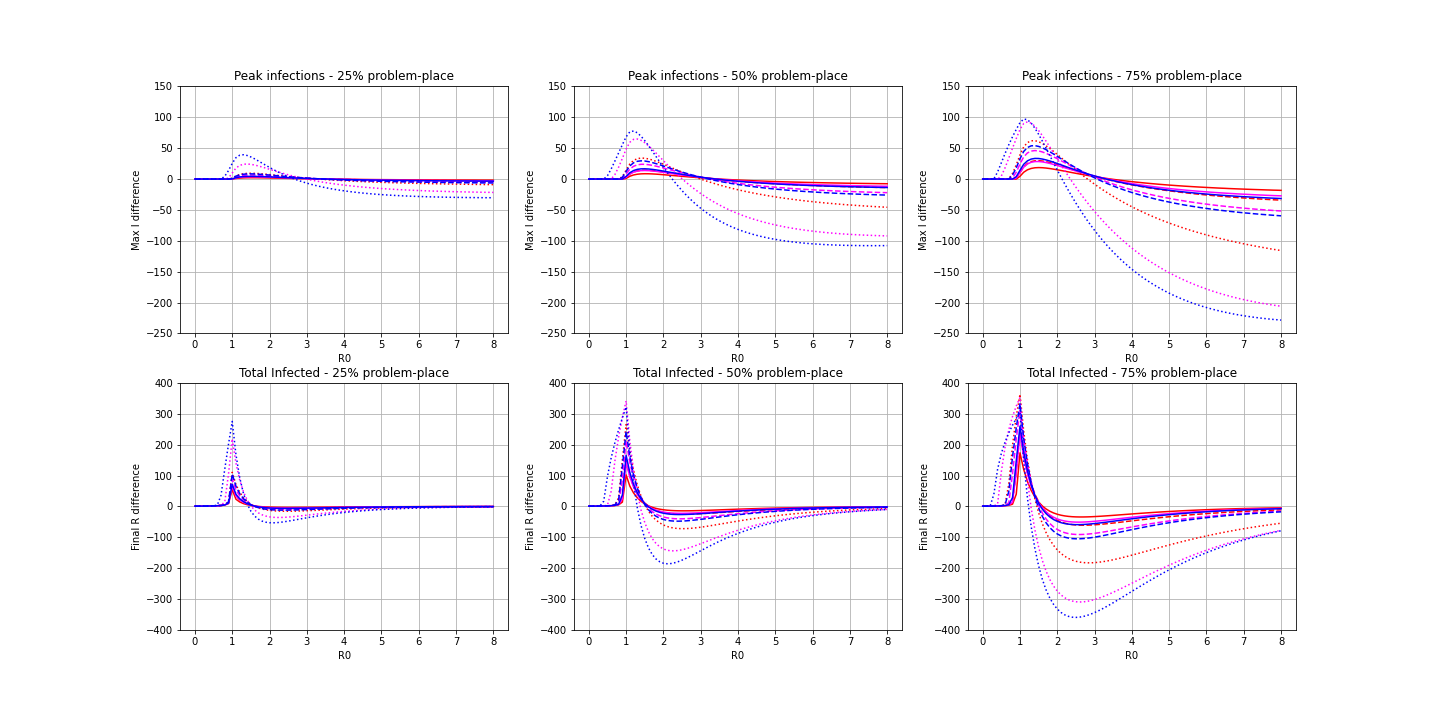
\includegraphics[width=\textwidth]{outbreakresults}
\caption{Outbreak Results}
\label{fig:outbreak_results}
\end{figure}

% \pagebreak
% outcome                  low R0       medium R0    high R0
% ---------------------   -------      ---------    --------
% outbreak probability    decreased     decreased    decreased
% peak infections         _increased_    _increased_    decreased
% total infections        _increased_    decreased    decreased

\subsection{Disease Evolution}

How can we explain these findings?

Here the differential equation model is useful.

In a more traditional compartment model, we can find $R(t)$ – the instantaneous
expected number of secondary infections caused by a new infection at time t.

In the analysis section we show that the basic reproduction number $R(t)$ is
given by:

$$R(t) = \frac{\bar S}{\gamma} \left( \beta_c
		+ \beta_r \bar \rho_S \bar \rho_I \right)$$

where $\bar\rho_S$ and $\bar\rho_I$ are the means of riskiness in the $S$ and
$I$ populations. We also show that


\begin{equation}
\frac{d\bar\rho_S}{dt} = 
\end{equation}

and

$$\frac{d\bar\rho_I}{dt} = ...$$

so that $\bar\rho_S$ always decreases at a rate proportional to the
variance of $\rho_S$ at the time, and that $\bar\rho_I$ is forced towards
some value between $\bar\rho_S$ and $\bar\rho_S + \frac{Var(\rho_S)}{\bar\rho_S}$
– which may be much larger than $\bar\rho_S$, but must necessarily increase
initially and later decrease.

If we plot the number of infected individuals during an outbreak alongside
$\mathcal{R}_t$ (\ref{fig:dynamics_comparison}), we see how this causes the
results from the previous section.

In the low $\mathcal{R}_0$ scenario, only a small outbreak was possible
under homogeneous dynamics; the acceleration causes a much higher spike by
comparison.\\

With a medium $\mathcal{R}_0$, problem-place dynamics shift the peak earlier
and it's higher.\\

With large $\mathcal{R}_0$, the peak is higher and lower than it would have
been under homogeneous dynamics.



%% TODO – would this be better with Rt plotted as well?
\begin{figure}
\centering
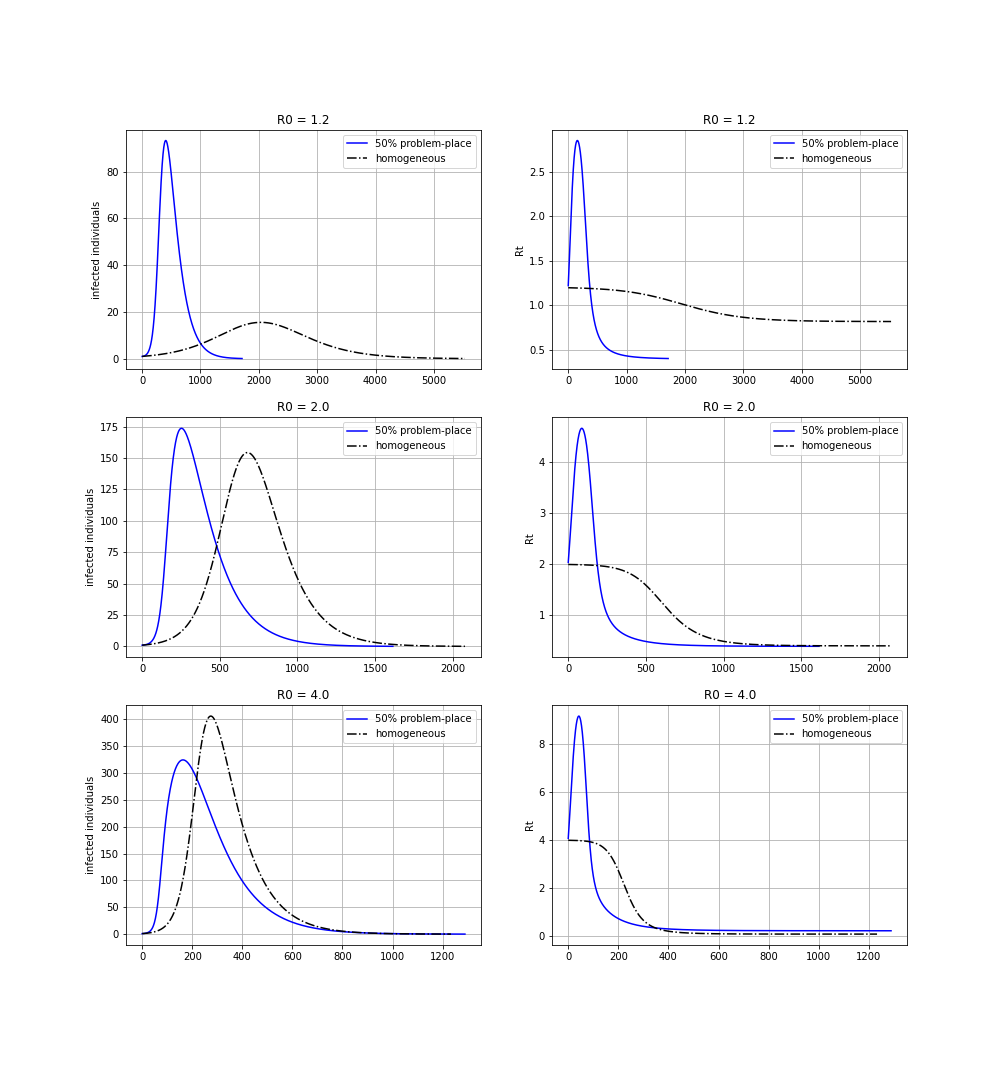
\includegraphics[width=\textwidth]{dynamics_comparison}
\caption{Dynamics Comparison}
\label{fig:dynamics_comparison}
\end{figure}


\pagebreak
\section{Analysis} 



\subsection{Disease Extinction}

\subsubsection{Homogeneous Case}

Given a disease with $\mathcal{R}_0$ of 2, the standard SIR model predicts an
outbreak to infect 79.681\% of the population before running its course.
When we simulate such an outbreak (\Cref{fig:extinction_histogram}) in
a population of 1,000, we see outbreaks of about this size, 
but we also see some number of simulations in which there's no large outbreak at all.\\

\begin{figure}
\centering
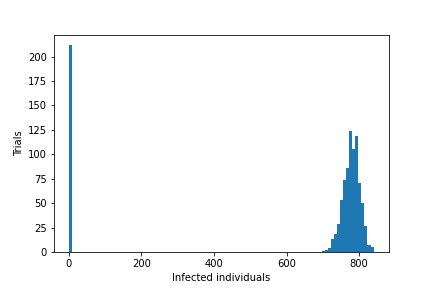
\includegraphics[width=0.6\textwidth]{extinction_histogram}
\caption{\textbf{Homogeneous Outbreak Sizes:} in each simulation, one individual
is initially  infected in a population of 1,000 with $\beta = 0.002$ so that
$\mathcal{R}_0$ = 2. We follow the simulation until no individuals are infected
and plot the number of total recovered individuals (i.e. total ever infected).} 
\label{fig:extinction_histogram}
\end{figure}


%![Figure 1. figure showing histogram of outbreak sizes](images/extinction_histogram.png)

We can predict the probability of a large vs small outbreak with reasonable
accuracy by replacing the outbreak scenario with a similarly parameterized
\textit{branching process}, and then asking how likely this branching process
is to go \textit{extinct}. This probability $\gamma$ is a function of
$p(n)$ – the probability of one individual infecting $n$ individuals before recovering:

$$
\gamma = p(0) + p(1) \gamma + p(2) \gamma^2 + ... + p(N) \gamma^N\\
$${

In the approximation, $p(n)$ is exactly the probability mass function
of a Binomial distribution with parameters $\beta$ and $N$, so the RHS of
the equation above is the generating function of the binomial distribution,
which gives:

$$
\gamma = (1 - \beta + \beta \gamma)^N\\
$$



This allows us to quite accurately predict the probability of a large outbreak
for any value of $\mathcal{R}_0$ and compare to the simulated results.
We show this in \Cref{fig:extinction_homogeneous}.

\begin{figure}
\centering
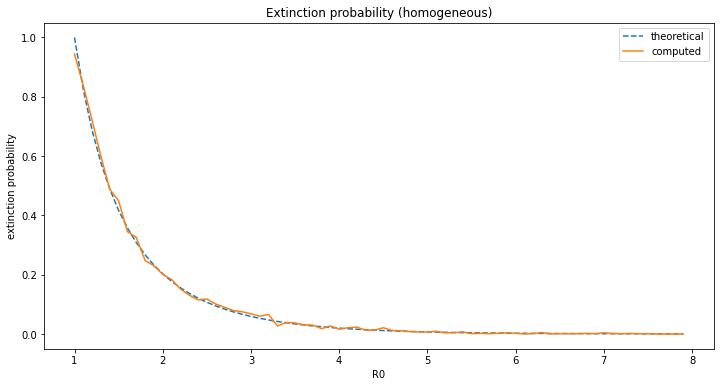
\includegraphics[width=0.6\textwidth]{extinction_homogeneous}
\caption{\textbf{Homogeneous Extinction Probabilities:} } 
\label{fig:extinction_homogeneous}
\end{figure}


\subsubsection{Problem-place}

Here we show that we can apply the same branching process approximation
to the problem-place model to predict the probability of a large outbreak
under any set of parameters.

Let X be a random variable that represents the number of infections caused by
a single infected individual with riskyness $\rho_i$ before recovering, and
let $j = 1, \ldots, N$ index the susceptible population so that $\rho_j$ is the
riskyness of individual $j$.

Then 
$$P(X = 0) = (1 - \rho_i) [ (1 - \beta_c)^N ] + \rho_i [ \prod_j (1 - (\beta_c + \beta_r \rho_j)) ]$$

By assumption riskyness for each individual is drawn independently from one
distribution, so in expectation (over riskyness values) this is:


\begin{align*}
E[P(X = 0)] &= E[(1 - \rho_i) [ (1 - \beta_c)^N ] + \rho_i [ \prod_j (1 - (\beta_c + \beta_r \rho_j)) ]]\\
&= (1 - E[\rho_i]) [ (1 - \beta_c)^N ] + E[\rho_i] [ \prod_j (1 - (\beta_c + \beta_r E[\rho_j])) ]]\\
&= (1 - \bar\rho) [ (1 - \beta_c)^N ] + \bar\rho [(1 - (\beta_c + \beta_r \bar\rho))^N ]\\
&= (1 - \bar\rho) B(\beta_c, N, 0) + \bar\rho B(\beta_c + \bar\rho \beta_r, N, 0)\\
\end{align*}

Where $B(a, b, x)$ is the Binomial probability mass at x with parameters a and b.

Similarly, $E[P(X) = x]$ is given by

$$(1 - \bar\rho) B(\beta_c, N, x) + \bar\rho B(\beta_c + \bar\rho \beta_r, N, x)$$


So


\begin{align*}
G_X(s) &= P(X=0) + P(X=1)s + P(X=2)s^2 + \ldots\\
&= [\bar\rho B_1(0) + (1 - \bar\rho)B_2(0)] + [\bar\rho B_1(1) + (1 - \bar\rho)B_2(1)]s + [\bar\rho B_1(2) + (1 - \bar\rho)B_2(2)]s^2 + \ldots\\
&= \bar\rho G_{B_1}(s) + (1 - \bar\rho)G_{B_2}(s)\\
&= \bar\rho [(1 - \bar\rho \beta_r)(1 - \beta_c) + 
				(1 - (1 - \bar\rho \beta_r)(1 - \beta_c) s]^N + 
   (1 - \bar\rho)[(1 - \beta_c) + \beta_c s]^N\\
\tau &= \bar\rho [(1 - \bar\rho \beta_r)(1 - \beta_c) + 
				(1 - (1 - \bar\rho \beta_r)(1 - \beta_c) \tau]^N + 
   (1 - \bar\rho)[(1 - \beta_c) + \beta_c \tau]^N\\
\end{align*}


% For small $\beta_c + \bar\rho \beta_r$, the overlap is very small so:

% $$ 
% \begin{aligned}
% P(X = x) &\approx (1 - \bar\rho) B(\beta_c, N, x) + \bar\rho (B(\beta_c, N, x) + B(\bar\rho \beta_r, N, x))\\
% &= \bar\rho B(\bar\rho \beta_r, N, x) + B(\beta_c, N, x)\\
% \end{aligned}
% $$

% And

% $$
% \begin{aligned}
% G_X(s) &\approx \bar\rho [(1 - \bar\rho \beta_r) + 
% 				\bar\rho \beta_r s]^N + [(1 - \beta_c) + \beta_c s]^N\\
% \tau &\approx \bar\rho [(1 - \bar\rho \beta_r) + 
% 				\bar\rho \beta_r \tau]^N + [(1 - \beta_c) + \beta_c \tau]^N
% \end{aligned}
% $$

\subsection{Outbreak Dynamics}

\subsubsection{Some initial definitions/conveniences}

Initial equations:


\begin{align*}
\frac{\partial S(\rho, t)}{\partial t} &=
	-\beta_c S(\rho, t) \int_{0}^1 I(u, t) du
	-\beta_r S(\rho, t) \rho \int_{0}^1 I(u, t) u du\\
\frac{\partial I(\rho, t)}{\partial t} &=
	\beta_c S(\rho, t) \int_{0}^1 I(u, t) du
	+ \beta_r S(\rho, t) \rho \int_{0}^1 I(u, t) u du - \gamma I(p, t)
\end{align*}


For convenience, we introduce the following shorthands 
for the "moments" of $I(\rho)$ and $S(\rho)$:


\begin{align*}
\bar S &:= \int_{0}^{1} S(\rho) d\rho
	& \bar I &:= \int_{0}^{1} I(\rho) d\rho\\
\hat S &:= \int_{0}^{1} S(\rho) \rho d\rho
	& \hat I &:= \int_{0}^{1} I(\rho) \rho d\rho\\
\hat{\hat{ S}} &:= \int_{0}^{1} S(\rho) \rho^2 d\rho
	& \hat{\hat{ I}} &:= \int_{0}^{1} I(\rho) \rho^2 d\rho\\
\vdots & & \vdots \\
\overset{(n)}{S} &:= \int_{0}^{1} S(\rho) \rho^n d\rho
	& \overset{(n)}{I} &:= \int_{0}^{1} I(\rho) \rho^n d\rho\\
\end{align*}


Now we can more concicely write the initial equations:


\begin{align*}
\frac{\partial S(\rho, t)}{\partial t} &=
	-\beta_c S(\rho, t) \bar I
	-\beta_r S(\rho, t) \rho \hat I\\
\frac{\partial I(\rho, t)}{\partial t} &=
	\beta_c S(\rho, t) \bar I
	+ \beta_r S(\rho, t) \rho \hat I - \gamma I(p, t)
\end{align*}


Finally, notice that $S(\rho)$ and $I(\rho)$ are defined over $\rho \in [0, 1]$,
and that these give the population at a given risk level. We can equivalently
think of how risk is distributed over the S and I populations:\\

We introduce $\rho_S$ and $\rho_I$: these are random variables drawn from
the distributions of risk in the S and I populations, respectively.

The means of these variables are:

\begin{align*}
\bar\rho_S
&= \frac{\int_{0}^{1} S(\rho) \rho d\rho}{\int_{0}^{1} S(\rho) d\rho}
= \frac{\hat S}{\bar S}\\
\bar\rho_I
&= \frac{\int_{0}^{1} I(\rho) \rho d\rho}{\int_{0}^{1} I(\rho) d\rho}
= \frac{\hat I}{\bar I}\\
\end{align*}

(This is just setting up interpretable variables for the terms
$\frac{\hat S}{\bar S}$ and $\frac{\hat I}{\bar I}$, which start to pop up
in a bunch of places.)\\


\subsubsection{Moments equations}

First we have a general result relating the "moments" of S and I.

% TODO - arrive at this by integration (maybe start with the 0)

Suppose we want to know how the total susceptible population is changing. We
can integrate $\frac{\partial S}{\partial t}$ over $\rho$:

\begin{align*}
\frac{d \bar{S}}{dt} = \int_{0}^{1} \frac{\partial S(\rho)}{\partial t} d\rho
&= \int_{0}^{1} (-\beta_c S(\rho) \bar I - \beta_r S(\rho) \rho \hat I) d\rho  \\
&= -\beta_c (\int_{0}^{1} S(\rho) d\rho) \bar I
	- \beta_r (\int_{0}^{1} S(\rho) \rho d\rho) \hat I\\
&= -\beta_c \bar S \bar I - \beta_r \hat S \hat I
\end{align*}

Similary, we can find that:

$$\frac{d \bar{I}}{dt} = \int_{0}^{1} \frac{\partial I(\rho)}{\partial t} d\rho
= \beta_c \bar S \bar I + \beta_r \hat S \hat I - \gamma \bar I$$\\

If we want to see how the first moments are changing, we follow a similar method:

\begin{align*}
\frac{d \hat{S}}{dt} = \int_{0}^{1} \frac{\partial S(\rho)}{\partial t} \rho d\rho
&= \int_{0}^{1} (-\beta_c S(\rho) \bar I - \beta_r S(\rho) \rho \hat I) \rho d\rho  \\
&= -\beta_c (\int_{0}^{1} S(\rho) \rho d\rho) \bar I
	- \beta_r (\int_{0}^{1} S(\rho) \rho^2 d\rho) \hat I\\
&= -\beta_c \hat S \bar I - \beta_r \hat{\hat{ S}} \hat I
\end{align*}\\

And for any general moment:


\begin{equation}
\label{eqn:moments}
\begin{aligned}
\frac{d \overset{(n)}{S} }{dt} &=
	-\beta_c \overset{(n)}{S} \bar I
	-\beta_r \overset{(n+1)}{S} \rho \hat I \\
\frac{d \overset{(n)}{I}}{dt} &=
	\beta_c \overset{(n)}{S} \bar I
	+ \beta_r \overset{(n+1)}{S} \rho \hat I - \gamma \overset{(n)}{I}
\end{aligned}
\end{equation}


\subsubsection{Basic Reproduction Number}

In the homogeneous SIR model, the basic reproduction number (number of secondary
infections per infection) is:

$$\mathcal{R}_t = \frac{S\beta}{\gamma}$$

In this model, we can derive a similar form for the expected
number of secondary infections per infection by dividing $\frac{d \bar S}{dt}$
by $\hat I$ (current number of infected individuals) then multiplying by
the mean duration of an infection $\frac{1}{\gamma}$.

\begin{align*}
\mathcal{R}_t &= -\frac{d\bar S}{dt} \frac{1}{\gamma \bar I} \\
	&= \frac{1}{\gamma} \beta_c \bar S \frac{\bar I}{\bar I}
		+ \frac{1}{\gamma} \beta_r \hat S \frac{\hat I}{\bar I}\\
	&= \frac{1}{\gamma} \bar S\left( \beta_c
		+ \beta_r \frac{\hat S}{\bar S} \frac{\hat I}{\bar I} \right)\\
	&= \frac{1}{\gamma} \bar S\left( \beta_c
		+ \beta_r \bar \rho_S \bar \rho_I \right)\\
\end{align*}

This gives a nicely analogous result, where the homogenous $\beta$ is
replaced by what we can think of as an effective $\beta$:
$(\beta_c + \beta_r \bar \rho_I \bar\rho_S)$, which is a straightforward
function of both $\beta$ terms and the mean riskiness in both populations.\\

We then would like to know how $\bar\rho_S$ and $\bar\rho_I$ are changing.
We'd expect $\bar\rho_S$ (mean riskiness of the susceptible population) to
monotonically decrease, as more risk-taking- susceptible individuals are
more likely to be infected. We'd expect $\bar\rho_I$ to behave almost
like a chemostat as higher-risk- individuals flow in, and all individuals flow
out at a rate of $\gamma$. It should increase initially, and eventually decrease
after the mean of riskiness decreases sufficiently in the susceptible population.

\subsubsection{Mean Susceptible Riskiness}

Fortunately, we can find explicit expressions for $\frac{d}{dt}\bar\rho_S$
and $\frac{d}{dt}\bar\rho_I$.\\

Start with $\frac{d\bar\rho_S}{dt}$, and differentiate:


\begin{align*}
\frac{d}{dt}\bar\rho_S
&= \frac{d}{dt} \left( \frac{\hat S}{\bar S} \right)\\
&= \frac{\frac{d}{dt} \hat S \bar S - \hat S \frac{d}{dt}\bar S}{\bar S^2}\\
&= \frac{1}{\bar S}\left(
-\beta_c\hat S \bar I - \beta_r \hat{\hat{S}}\hat I
\right)
- \frac{\hat S}{\bar S^2}\left(
-\beta_c \bar S \bar I - \beta_r \hat S \hat I
\right)\\
&= -\beta_c \frac{\hat S}{\bar S} \bar I
- \beta_r \frac{\hat{\hat{S}}}{\bar S}\hat{I}
+ \beta_c \frac{\hat S}{\bar S}\bar I
+ \beta_r \left(\frac{\hat S}{\bar S}\right)^2 \\
&= 
- \beta_r \frac{\hat{\hat{S}}}{\bar S}\hat{I}
+ \beta_r \left(\frac{\hat S}{\bar S}\right)^2 \\
&= -\beta_r \hat I \left(\frac{\hat{ \hat{ S}}}{\bar S} - \left(\frac{\hat S}{\bar S}\right)^2  \right)\\
\end{align*}

Here, notice $\hat{ \hat{ S}}$ sums $\rho^2$ over $[0, 1]$ and so
$\frac{\hat{ \hat{ S}}}{\bar S}$ we can write as $E[\rho_S^2]$. And similarly
$\frac{\hat S}{\bar S}$ = $E[\rho_S]$ so
$$
\frac{\hat{ \hat{ S}}}{\bar S} - \left(\frac{\hat S}{\bar S}\right)^2
= E[\rho_S^2] - E[\rho_S]^2 
$$

which is the variance of the riskiness of the susceptible population
$Var(\rho_S)$. This allows us to rewrite the equation as:

$$
\frac{d}{dt}\bar\rho_S = -\beta_r \hat I \text{Var}(\rho_s)
$$

or

$$
\frac{d}{dt}\bar\rho_S = -\beta_r \bar I \bar\rho_I \text{Var}(\rho_s)
$$

This confirms that $\rho_S$ decreases monotonically (as long as there is some
infected population with nonzero mean riskiness), and further shows that
it decreases proportionally to the variance of the distribution of riskiness
in the S population.

\subsubsection{Mean Infected Riskiness}


% TODO - add all the stuff after applying product rule

\begin{align*}
\frac{d}{dt}\bar\rho_I
&= \frac{d}{dt} \left( \frac{\hat I}{\bar I} \right)\\
&= \frac{\frac{d}{dt} (\hat I) \bar I - \hat I \frac{d}{dt}(\bar I)}{\bar I^2}\\
&=  ...
\\
&= \bar S \left[
	\beta_c (\bar\rho_S - \bar\rho_I)
	+ \beta_r \bar\rho_S \bar\rho_I((\bar\rho_S + \frac{\text{Var}(\rho_S)}{\bar\rho_S})
		- \bar\rho_I))
\right]
\end{align*}
\end{document}
